\documentclass[a4paper,10pt]{article}
\usepackage[utf8]{inputenc}

%opening
\title{}
\author{}

\usepackage{amsmath,amssymb,amsfonts,amsthm,mathtools} % Mathematik

\usepackage{color}

\begin{document}

\section*{Task 7}

\noindent Gauss Legendre quadrature is a quadrature rule where the evaluation points are the roots of the
$n$-th Legendre polynomial and the weights are the integrals of the corresponding Lagrange polynomials of degree $n$ over the integration domain.\\

\noindent Legendre polynomial:
\begin{align*}
 P_n(x)&=\frac{1}{2^n}\sum_{k=0}^n {n \choose k}^2 (x-1)^{n-k}(x+1)^k \\
 &= \sum_{k=0}^n {n \choose k}{-n-1 \choose k}\left(\frac{1-x}{2}\right)^k
\end{align*}

\noindent Lagrange polynomials:
\begin{align*}
 L_{i,n}(x)=\prod_{j=0 \atop j\neq i}^n \frac{x-x_j}{x_i-x_j}
\end{align*}
(Where $x_i$ are the evaluation points.)

\subsection*{Level behavior}
We concluded that the behavior of the nodes does not change likewise as in the other integrating methods. We see in the graphic below that the roots of the polynomials do not cross.
\begin{figure}[htbp]
	\centering
		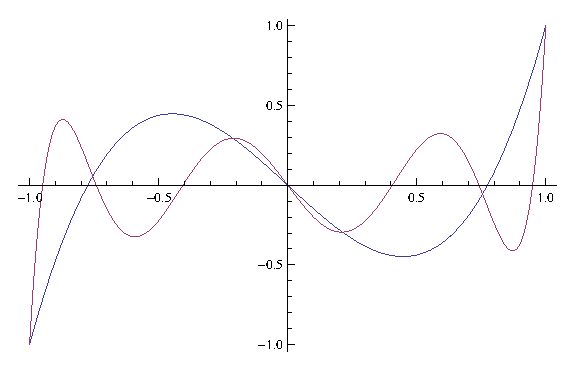
\includegraphics[width=1.00\textwidth]{F:/LevelBehavior.eps}
	\caption{LevelBehavior}
	\label{fig:LevelBehavior}
\end{figure}

% \noindent To proof:
% \begin{align*}
%  \frac{1}{\sqrt{2 \pi}} \int_{-\infty}^\infty f(s)e^{-\frac{s^2}{2}}ds =& \int_{0}^1 f(\Phi^{-1}(t))dt
% \end{align*}
% Proof:
% \begin{align*}
%  \frac{1}{\sqrt{2 \pi}} \int_{-\infty}^\infty f(s)e^{-\frac{s^2}{2}}ds =& \lim_{a\rightarrow \infty}\int_{-a}^a f(s) \phi '(s)ds\\
%   =& \lim_{a\rightarrow \infty}\int_{\Phi(-a)}^{\Phi(a)} f(\Phi^{-1}(t)) dt\\
%   =& \int_{0}^{1} f(\Phi^{-1}(t)) dt
% \end{align*}
% With substitution $s\rightarrow \Phi^{-1}(t)$.
% \flushright{$\qed$}


\end{document}
